Las técnicas de clustering jerárquico son, como las de clustering particional, relativamente antiguas en comparación con muchas otras que analizaremos más adelante.
Aún así se mantienen entre las más usadas en la actualidad.
Fueron desarrolladas con la finalidad de resolver algunas de las desventajas de los algoritmos de clustering particional que hemos visto, como su necesidad de una cantidad de clusters prefijada y su naturaleza no determinista.

Existen dos clasificaciones para los algoritmos de clustering jerárquico de acuerdo al modo de generar los clusters:

\begin{itemize}
    \item \textbf{Aglomerativos}: Cada punto comienza en un cluster propio y, en cada paso, se une el par de clusters más próximos entre sí.
    Requiere la definición de una medida para la proximidad entre clusters.
    \item \textbf{Divisivos}: Se comienza con un único cluster que contiene a todos los puntos y, en cada paso, se divide un cluster hasta obtener clusters de solamente un elemento.
    Requiere un criterio para decidir cuál cluster dividir en cada paso y cómo redistribuir a sus miembros entre los dos clusters resultantes.
\end{itemize}

Debido al modo en que se ejecutan los algoritmos de clustering jerárquico, su ejecución sobre un conjunto de datos puede ser visualizado gráficamente mediante diagramas llamados \textit{dendrogramas}, que representan las relaciones entre cada cluster y los sub-clusters formados a partir de este durante los distintos pasos del algoritmo.

Las técnicas de clustering aglomerativas son las más estudiadas~\cite{Tan05}, y serán las que abordaremos en esta sección.

\begin{algorithm}
    \caption{Clustering aglomerativo}
    \label{algorithm:clusteringAglomerativo}
    Computar la matriz de proximidad si es necesario\;
    \Repeat{Solo queda un cluster}{
    Unir los dos clusters más próximos\;
    Actualizar la matriz de proximidad en correspondencia con las distancias entre el nuevo cluster y los ya existentes\;
    }
\end{algorithm}

\subsection{Proximidad entre clusters}\label{subsec:proximidadEntreClusters}

Resulta clave para el funcionamiento del algoritmo~\ref{algorithm:clusteringAglomerativo} el cálculo de la proximidad, o distancia, entre dos clusters.
Este concepto constituye la diferencia entre los distintos algoritmos de clustering aglomerativo, siendo los dos siguientes los métodos más populares~\cite{Aggarawal13}:

\begin{itemize}
    \item \textbf{Single link}: La distancia, o similaridad, entre dos clusters es la distancia entre sus miembros más cercanos entre sí.
    Este método prioriza las regiones en que los clusters son más próximos, sin tener en cuenta la estructura global de estos.
    \item \textbf{Complete link}: La similaridad entre dos clusters se mide por la distancia entre sus miembros más alejados entre sí.
    Esto es equivalente a seleccionar el par de clusters que minimiza el diámetro del resultado de su unión, produciendo clusters compactos generalmente.
\end{itemize}

\begin{figure}[!h]
    \centering
    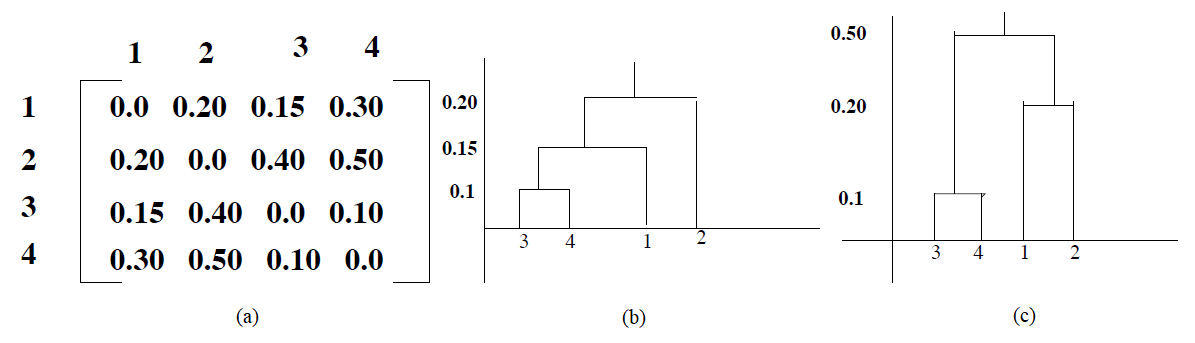
\includegraphics[width=\textwidth]{agglomerative-clustering.png}
    \caption{Ejemplo de aplicación de algoritmos de clustering aglomerativo. (a) Matriz de similaridad para un conjunto de datos de 4 puntos.
    Dendrogramas obtenidos a partir de este conjunto usando los métodos de clustering aglomerativo (b) single link y (c) complete link. (Tomado de~\cite{Aggarawal13}.)}
\end{figure}

\textbf{Group averaged}~\footnote{También conocido como \textit{Average linkage}} es una tercera variante de clustering aglomerativo.
En este caso, la similitud entre dos clusters no es determinada por la distancia entre dos puntos específicos de estos, sino por el promedio de todas las distancias punto a punto entre los dos clusters.
Se caracteriza por requerir una complejidad de cálculos mayor que las dos variantes anteriormente mencionadas, lo que hace que sea menos usada.
Una variación que busca compensar esta dificultad es la técnica nombrada \textbf{Centroid-based agglomerative clustering}~\footnote{\textit{Clustering aglomerativo basado en centroides} en español}, que determina la distancia entre dos clusters a partir de sus respectivos centroides.

\subsubsection{Método de Ward}

El método de Ward es una propuesta para el cálculo de la distancia entre dos clusters usado en el clustering aglomerativo.
Utiliza la ecuación~(\ref{eq:SSE}) de la SSE para medir la distancia entre dos clusters como el incremento que produce en este valor unir dichos clusters.
Al igual que K-Means, este método intenta minimizar la suma de las distancias al cuadrado de cada punto al centroide de su cluster.

\subsubsection{Complejidad espacial y temporal}

La matriz de proximidad usada por los algoritmos de clustering jerárquico aglomerativos requiere el almacenamiento de $\frac{1}{2}n^2$ valores (asumiendo que la matriz es simétrica), donde $n$ es la cantidad de observaciones presentes en los datos.
El espacio necesario para almacenar el registro de los clusters es proporcional al número de estos, que es menor o igual que $n$.
La complejidad de memoria requerida por estos algoritmos es, por tanto, $O(n^2)$.

En cuanto al tiempo, el cálculo de la matriz de distancias es $O(n^2)$.
Los pasos 3 y 4 requieren $n-1$ iteraciones puesto que existen $n$ clusters al comienzo, y en cada paso se unen dos, reduciéndose en uno la cantidad de clusters en cada momento.
Si el paso 3 es realizado como una búsqueda lineal sobre la matriz, entonces este requerirá un tiempo $O((n-i+1)^2)$ en la $i$-ésima iteración.
El paso 4 solo requiere un tiempo $O(n-i+1)$ para actualizar la matriz luego de unir dos clusters.
Sin efectuar ninguna modificación, esto nos lleva a una complejidad temporal total $O(n^3)$.
Aunque aplicando mejoras como el empleo de estructuras de datos alternativas para almacenar la matriz y optimizar la búsqueda del paso 3, esta complejidad puede disminuirse hasta $O(n^2\log{n})$~\cite{Tan05}.

La complejidad espacial y temporal de los algoritmos de clustering jerárquico constituye una de las principales limitantes para su empleo sobre conjuntos de datos de tamaño significativo.